\documentclass[runningheads]{llncs}

% ===== GRAPHICS AND COLORS =====
\usepackage{graphicx}
\usepackage[usenames,dvipsnames]{xcolor}
\usepackage{booktabs, multirow, colortbl}
\usepackage{fontawesome5}
\usepackage{amssymb}
\usepackage{verbatimbox}
\usepackage{float}

% ===== TABLES =====
\usepackage{array}

% ===== FIGURES AND TIKZ =====
\usepackage{tikz}
\usetikzlibrary{arrows.meta, positioning, matrix}

% ===== ALGORITHMS =====
\usepackage{algorithm}
\usepackage{algorithmic}

% ===== HYPERLINKS (load before bidi) =====
\usepackage[hidelinks]{hyperref}
\usepackage{url}

% ===== CODE LISTINGS =====
\usepackage{listings}
\lstset{
  basicstyle=\small\ttfamily,
  breaklines=true,
  escapeinside={(*}{*)}
}


% ===== PERSIAN SCRIPT SUPPORT =====
\usepackage{xspace}
\usepackage{fontspec}
\usepackage[english,main=english]{babel}
\babelprovide[import=ar, onchar=ids fonts]{arabic}
\babelfont[arabic]{rm}{Amiri}   % more integrated than \newfontfamily

% For short Persian phrases (no extra space, no break)
\newcommand{\textfarsi}[1]{{\foreignlanguage{arabic}{#1}}\xspace}
% \makeatletter
%\def\bibsection{\section*{References}}
%\makeatother
% ===== DOCUMENT SPACING =====
\raggedbottom

\begin{document}

\title{Scaling Fine-Grained Emotion Classification for Farsi-Dari: A Semi-Supervised Pipeline and a New 400k-Entry Social Media Corpus}
\titlerunning{DEEP-Dari: Scaling Emotion Classification for Farsi-Dari}
\author{Azizullah Massomy \and Werner Winiwarter\and Dominik Dolezal }
\authorrunning{A. Massomy et al.}
\institute{University of Vienna, Faculty of Computer Science,\\
W\"{a}hringerstra{\ss}e 29, 1090 Vienna, Austria\\
\href{mailto:massomya22@univie.ac.at}{\texttt{massomya22@univie.ac.at}}, 
\href{mailto:werner.winiwarter@univie.ac.at}{\texttt{werner.winiwarter@univie.ac.at}}, 
\href{mailto:dominik.dolezal@univie.ac.at}{\texttt{dominik.dolezal@univie.ac.at}}\\
}

\date{}
\maketitle

\begin{abstract}
 Sentiment analysis is well-established for major languages, but dialectal variants like Farsi-Dari still lack the basic resources needed for high-quality research. This is especially true for fine-grained emotion detection, where labeled data is nearly non-existent. In this paper, we address this resource gap by developing a semi-supervised pipeline. We first fine-tune a ParsBERT model on a manually annotated set of 3932 samples to serve as a high-quality labeling agent, which is then used to automatically annotate a larger corpus of over 391,691 social media posts and comments from Telegram and YouTube. A major challenge was the extreme lack of ``Fear" samples, which made up less than 1\% of the original data. By applying targeted data augmentation and adding a new "Hope" category to reflect local social discourse, we increased model accuracy from a 50.57\% baseline to 85.75\%. Our work shows that even with very few initial labels, it is possible to build high-performing emotion models for low-resource languages by using smart scaling and cultural context.


\end{abstract}
\keywords{Emotion Classification \and Dari Social Media \and Semi-Supervised Learning \and Data Augmentation \and Sociolinguistics  \and Low-Resource NLP \and Emotion Detection \and Diglossia \and Large-Scale Corpus.}
\section{Introduction}

The digital landscape of social media has created an unprecedented volume of 
unstructured data, with approximately 80-90\% of modern text consisting of 
informal logs, chat messages, and user-generated content\footnote{Aparavi (2025): 80-90\% of data is unstructured. \url{https://aparavi.com/resources/blog/preparing-unstructured-data-for-ai/}}.
While sentiment analysis has reached high maturity for languages with vast 
linguistic resources, regional variants such as Dari (Afghan Persian) remain 
significantly underserved. This discrepancy is not merely a technical 
oversight but a sociolinguistic one; Dari serves as the primary vehicle for 
the digital public square in Afghanistan and its global diaspora\footnote{Kabul Times (2024): 6.5M Afghans live abroad. \url{https://thekabultimes.com/refugees-challenges-ahead/.}}.

In regions where traditional polling and physical public discourse are often 
restricted, social media platforms like Telegram and YouTube become vital 
archives of the collective mood, harboring deep-seated social reflections 
that are otherwise inaccessible. Dari is not merely a geographic dialect but 
a distinct linguistic entity with unique slang, emotional triggers, and 
cultural nuances that standard Persian models often fail to capture. 
Linguistically, Dari retains archaic lexical features and distinct 
socio-pragmatic markers~\cite{baker2016dari}—particularly in how grief, resilience, and honor are 
expressed—that require a culturally situated approach to sentiment rather 
than a generic translated framework. The analysis of Dari digital discourse 
provides a dual lens: a linguistic record of how the language evolves in 
informal spaces and a social record of the global Afghan diaspora's 
collective mood. By tracking these developments at both a linguistic and 
social level, we can observe how the community maintains cultural continuity 
while reacting to shifting home-country conditions.

The primary challenge in analyzing Dari social media is the ``resource gap''. Existing datasets are often small, poorly 
cleaned, or translated from English, which strips away the cultural context. 
Such translation-based models frequently ignore the social reality that 
emotions are not universal constants but are filtered through a specific 
cultural lens. Furthermore, fine-grained emotion detection—moving beyond 
simple positive/negative polarity~\cite{mudiyanselage2026context}—is 
hindered by extreme class imbalance. In natural discourse, critical emotions 
like ``Fear'' or specialized categories like ``Hope'' are rare, often 
representing less than 1\% of naturally occurring data~\cite{kumar2025longtail}. Yet, from a social 
analysis perspective, these minority classes are often the most significant, 
providing early indicators of social shifts or humanitarian needs.

In this paper, we address these limitations by proposing a semi-supervised 
pipeline designed to scale emotion classification for Dari. Our approach 
moves away from a total reliance on scarce manual labor. Instead, we use a
Native-Speakers ``Gold Standard'' set of 3,932 manually labeled samples to 
fine-tune a ParsBERT transformer model~\cite{farahani2021parsbert}. This 
fine-tuned model then acts as an expert labeling agent, allowing us to 
bootstrap and automatically annotate a massive corpus of over 391,691 
entries from Telegram and YouTube. To ensure the integrity of the data and 
counter the ``curse of knowledge,'' we employ a targeted data augmentation 
strategy (Sect.~\ref{sec:arg}) that revitalizes minority classes, ensuring that 
rare but significant emotions are not lost to the model.

The primary contributions of our work are as follows:

\begin{itemize}
    \item \textbf{Novel 400k-Entry Corpus:} We introduce the largest known 
    emotion-labeled dataset for Dari social media, providing a robust 
    benchmark for low-resource NLP.
    
    \item \textbf{High-Precision Semi-Supervised Pipeline:} We demonstrate 
    that fine-tuning a transformer on a small, expert-curated set can 
    effectively label large-scale noisy data with an accuracy of 85.75\%.
    
    \item \textbf{Culturally-Informed Emotion Modeling:} By integrating a 
    specialized ``Hope'' category, we capture the optimistic socio-political 
    discourse prevalent in Afghan digital communities, which is missing from 
    standard models.
\end{itemize}

The remainder of this paper is organized as follows. Section 2 discusses the 
linguistic landscape of Farsi-Dari. Section 3 reviews the relevant literature 
on Persian NLP and imbalanced learning. Section 4 details our semi-supervised 
methodology and data collection. Section 5 presents the experimental setup, 
followed by a discussion and an analysis of results in Sect.~\ref{sec:results}. Finally, 
Section 7 concludes the paper. 
\section{Linguistic Background: Farsi vs. Dari}

Dari (Afghan Persian) and Iranian Persian share a common literary heritage 
but diverge significantly in social media discourse. While Farsi benefits from 
sophisticated NLP models like ParsBERT~\cite{farahani2021parsbert}, Dari remains 
underserved due to distinct socio-political vocabulary and diglossia---the gap 
between formal writing and informal online speech~\cite{mahmoodi2018spoken}. 

This diglossic gap is particularly pronounced in emotional expression. 
In formal Farsi, emotions are often conveyed through standardized literary 
constructions. In contrast, Dari speakers on social media employ colloquial 
forms, religious invocations, and culturally specific metaphors that have no 
direct Farsi equivalent. For example, expressions of ``Hope" in Dari frequently 
include future-tense aspirations for peace and reconstruction, such as 
\textfarsi{کند خدا}(God willing...), 
which standard Farsi models misclassify as neutral or happy.
As emphasized by Rooein et al.~\cite{rooein2025culturally}, culturally-grounded 
emotion modeling is essential for conflict-affected regions.
Applying Farsi models to Dari text causes a ``lexical mismatch'': regional slang, 
orthographic variation, and Pashto-derived emotional markers are frequently 
flagged as out-of-vocabulary~\cite{hussiny2024persianemo}. 
This mismatch is not merely technical but semantic: the emotional 
intensity of a Dari expression can be lost when forced into a Farsi-trained 
embedding space. Consequently, off-the-shelf Persian sentiment tools perform 
poorly on Dari social media, motivating our development of a dedicated pipeline.

We adopt Ekman's categorical emotion model~\cite{ekman1992} (Fear, Anger, Sadness, 
etc.), which provides higher interpretability for social analysis than 
dimensional frameworks. This categorical approach is particularly 
well-suited for conflict-zone social media analysis, where detecting specific 
high-arousal emotions (Fear, Anger) provides actionable insights for humanitarian 
monitoring. Unlike dimensional models that reduce emotions to valence-arousal 
coordinates, discrete categories align with how Dari speakers themselves 
conceptualize emotional states in everyday discourse.
Our linguistic assumptions are grounded in Cambridge profiles of Afghan Persian~\cite{baker2016dari}, documenting the phonetic shifts that cause orthographic instability in our corpus.

\section{Related Work}
\label{sec:rel_work}

The landscape of sentiment analysis has shifted significantly from lexicon-based approaches to deep transformer architectures. Early efforts in Persian sentiment analysis utilized traditional machine learning and shallow neural networks to overcome the limitations of manual feature engineering. For instance, Dashtipour et al.~\cite{dashtipour2018exploiting} demonstrated the efficacy of Convolutional Neural Networks (CNNs) and Deep Autoencoders for binary polarity detection (positive/negative) in Persian movie reviews, achieving accuracies up to 82\%. While these models established a baseline for deep learning in the region, they were primarily focused on structured, formal text and binary classification, leaving a gap in our understanding of fine-grained emotions in informal, dialectal social media environments.
\subsection{Persian/Dari Emotion Analysis}
Early research in Persian sentiment analysis primarily focused on binary polarity (positive/negative). With the advent of transformer-based models, the field has moved toward contextualized embeddings. Farahani et al.~\cite{farahani2021parsbert} introduced ParsBERT, which established a new state-of-the-art for Persian NLP tasks by leveraging a large-scale Persian corpus for pre-training. While ParsBERT has shown robustness in general sentiment tasks, recent surveys~\cite{abaskohi2022persian} indicate that its performance can be unstable when applied to informal social media text or specific dialects like Dari.

The ``resource gap" for Dari is particularly evident in fine-grained emotion modeling. A significant recent contribution in this area is PersianEmo by Hussiny et al.~\cite{hussiny2024persianemo}, which introduced the \textit{LearnArmanEmo}\footnote{LearnArmanEmo combines ARMANEMO (Persian tweets) and LetHerLearn (Dari comments). Their hybrid architecture uses XLM-RoBERTa (multilingual transformer) and BiGRU (bidirectional RNN).} dataset—a combination of the Farsi-based ARMANEMO and the Dari-specific \textit{LetHerLearn} corpus. Their hybrid XLM-RoBERTa and BiGRU architecture achieved F1-scores of 72.9\% on Dari text and 77.1\% on Farsi, utilizing a 7-class taxonomy: \textit{Anger, Disgust, Fear, Happiness, Sadness, Surprise,} and \textit{Other/Neutral}.

While PersianEmo provides a critical linguistic foundation, these existing frameworks often overlook the specific socio-political lexicon and emotional nuances of Afghan speakers. In this study, we extend the standard 7-class model into an 8-class framework by integrating a ``Hope" category. This addition is designed to capture a critical dimension of optimistic and aspirational discourse—common in diaspora communities and regional Dari commentary—which traditional models often misclassify as ``Neutral" or ``Happiness" due to the absence of a forward-looking affective label. By adapting the PersianEmo baseline to include this category, we aim to improve the cultural and semantic coverage of emotion detection in the Dari-speaking digital sphere.
Recent work by Muhammad et al.~\cite{muhammad2025brighter} confirms 
that fine-grained emotion classification across low-resource languages 
remains a significant challenge.


\subsection{ Scaling via Semi-Supervised Learning}
Manual annotation remains the ``gold standard" but is notoriously difficult to scale for low-resource languages. Recent studies in semi-supervised learning suggest that small, expert-curated ``seed" datasets can be used to bootstrap much larger corpora through self-training and pseudo-labeling. Sosea and Caragea~\cite{sosea2022leveraging} demonstrated that self-training with pseudo-labeling can significantly improve text classification performance in low-resource settings, achieving an average F1 improvement of 3.5\% over strong baselines. Our work follows this trajectory, using a fine-tuned ParsBERT model as an expert labeling agent to scale our dataset from 3,932 to over 391,691 entries.
\subsection{Challenges of Class Imbalance and Augmentation}

A persistent issue in fine-grained emotion detection is the extreme scarcity of
certain emotional states, such as Fear or Disgust, in natural social media dis-
course. Standard accuracy metrics often mask the failure of models to learn
these minority classes, necessitating the use of macro-F1 and detailed confusion
matrices \cite{cui2025addressing}. 

Mu et al.~\cite{mu2025limitations} demonstrated that loss reweighting alone is insufficient
for extreme class imbalance. Üveges and Ring~\cite{uveges2025synthetic} similarly found that synthetic data
generation significantly improves classification performance for minority emotion classes, though they note limitations such as reduced lexical diversity in
generated samples. Radliński et al.~\cite{radlinski2025backtranslation} systematically compared traditional
augmentation methods (backtranslation, paraphrasing) with LLM-based generation (ChatGPT),
finding that traditional methods can perform as well as or better than LLM generation
for low-resource emotion classification.

Recent findings suggest that augmentation is most effective when it is targeted
and culturally grounded \cite{nta2025augmentation}. This supports our decision to implement a targeted
augmentation strategy for the ``Fear'' class, using culturally relevant triggers specific
to the Dari-speaking context, thereby addressing the extreme class imbalance that standard weighting alone could not resolve.
\subsection{Distinction from Aspect-Based Sentiment Analysis (ABSA)}
A significant portion of Persian NLP literature is dedicated to Aspect-Based Sentiment Analysis (ABSA), which focuses on identifying polarities toward specific entities or products. However, our research prioritizes broad emotion detection. While ABSA is valuable for consumer insights, emotion detection is better suited for analyzing short-term reactions to geopolitical incidents and the long-term emotional resilience of conflict-affected populations. This approach allows us to capture the overarching `collective mood' rather than target-specific opinions.
\section{The Dari Emotion Expansion Pipeline}
\label{sec:methodology}
In this section, we describe the \textbf{Dari Emotion Expansion Pipeline (DEEP-Dari)}, a semi-supervised framework designed to scale expert linguistic intuition into a large-scale corpus. The workflow moves from a high-precision human-labeled seed to a robust, 390k-entry classifier. The overall architecture is summarized in Fig.
~\ref{fig:pipeline}.
\begin{figure}[H]
\centering
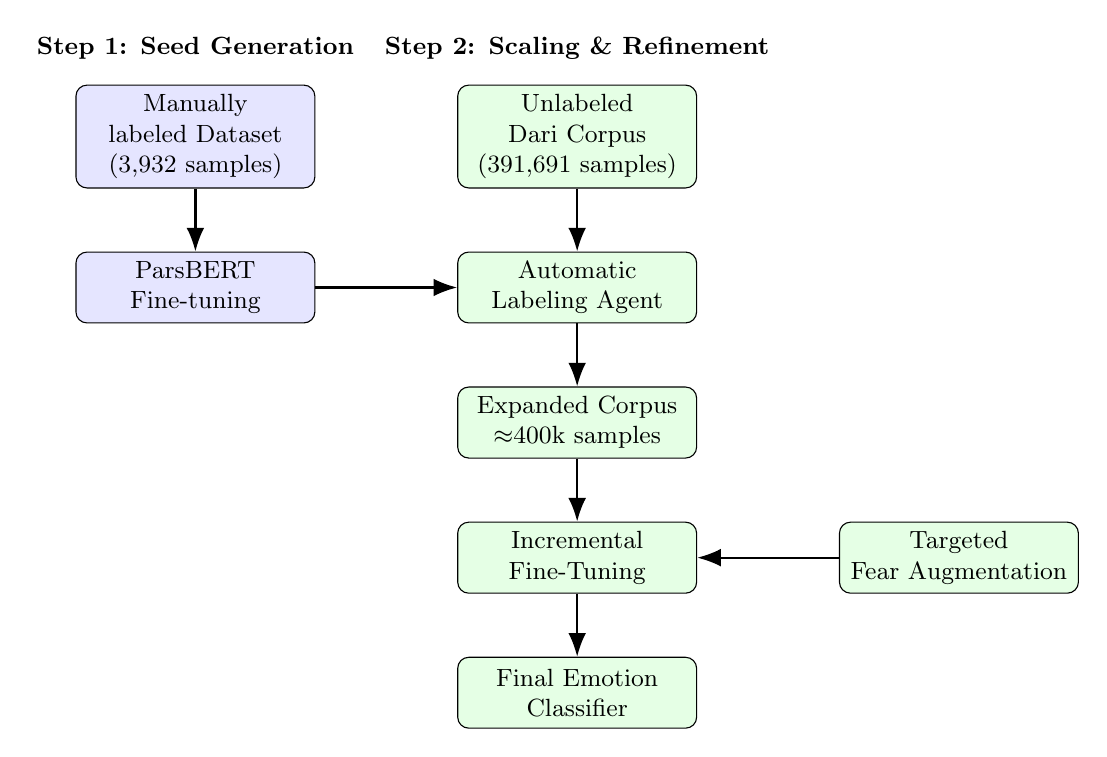
\begin{tikzpicture}[
    node distance=0.8cm and 1.8cm,
    block/.style={
        draw,
        rectangle,
        rounded corners=4pt,
        align=center,
        minimum width=3.0cm,
        minimum height=0.9cm,
        fill=blue!5,
        text width=2.8cm,
        font=\small
    },
    step1/.style={block, fill=blue!10},
    step2/.style={block, fill=green!10},
    arrow/.style={-{Latex[length=3mm]}, thick},
    label/.style={font=\small\bfseries}
]

% Step 1 nodes (The Seed)
\node[step1] (p1data) {Manually\\ labeled Dataset\\(3,932 samples)};
\node[step1, below=of p1data] (p1model) {ParsBERT\\Fine-tuning};

% Step 2 nodes (The Scaling)
\node[step2, right=of p1data] (unlabeled) {Unlabeled\\Dari Corpus\\(391,691 samples)};
\node[step2, below=of unlabeled] (autolabel) {Automatic\\Labeling Agent};
\node[step2, below=of autolabel] (expanded) {Expanded Corpus\\$\approx$400k samples};
\node[step2, below=of expanded] (finetune) {Incremental\\Fine-Tuning};
\node[step2, right=of finetune] (aug) {Targeted\\Fear Augmentation};
\node[step2, below=of finetune] (final) {Final Emotion\\Classifier};

% Step labels
\node[label, above=0.2cm of p1data] {Step 1: Seed Generation};
\node[label, above=0.2cm of unlabeled] {Step 2: Scaling \& Refinement};

% Arrows
\draw[arrow] (p1data) -- (p1model);
\draw[arrow] (p1model.east) -- ++(0.5,0) |- (autolabel.west);
\draw[arrow] (unlabeled) -- (autolabel);
\draw[arrow] (autolabel) -- (expanded);
\draw[arrow] (expanded) -- (finetune);
\draw[arrow] (aug) -- (finetune);
\draw[arrow] (finetune) -- (final);

\end{tikzpicture}
\caption{DEEP-Dari architecture: Seed generation (left) and scaling with augmentation (right).}
\label{fig:pipeline}
\end{figure}
The DEEP-Dari architecture, detailed in Fig.~\ref{fig:pipeline}, represents a semi-supervised knowledge transfer process. It moves from a small-scale, high-fidelity human seed to a large-scale, machine-annotated corpus. A key innovation in this pipeline is the parallel integration of targeted augmentation during the final fine-tuning phase, which prevents the model from being biased toward the majority classes (Happy/Neutral) prevalent in the raw social media feed.
\subsection{Multi-Source Data Acquisition}
We collected data from two main sources to capture the language of the Afghan diaspora and regional speakers.

\begin{itemize}
    \item \textbf{Telegram:} We searched for public groups using Dari keywords and also added a few manually selected high‑activity channels (one had over 8,000 members). This gave us 24,192 raw messages. After cleaning, 19,319 remained, with timestamps ranging from February 2017 to May 2025.
    \item \textbf{YouTube:} We scraped comments from five channels that cover political, cultural, and regional themes: \textit{Kaktos} (politics), \textit{Reza \& Fatima} (culture/region), \textit{NR} (general Dari discourse), \textit{BV} (general content), and \textit{People Media} (focused cultural commentary). The raw comments totalled 486,860\footnote{Raw (pre‑cleaning) totals: Telegram 24,192, Kaktos 198,511, Reza\&Fatima 181,514, NR 87,788, BV 17,963, People Media 1,084; combined raw total 511,052.}; after cleaning we kept 391,691.
\end{itemize}

After removing duplicates, Emojis, URLs, non‑Persian characters, and messages shorter than four words, the final cleaned dataset contains \textbf{391,691} messages, with an average length of \textbf{15.1} tokens per message. Table~\ref{tab:data_sources_detailed} gives the breakdown per source, including sample counts and date ranges.
\begin{table}[H]
\centering
\caption{Detailed breakdown of data sources.}
\label{tab:data_sources_detailed}
\begin{tabular}{@{}p{2.5cm}p{3cm}p{3.5cm}p{3.5cm}@{}}
\toprule
\textbf{Platform} & \textbf{Channel/Group} & \textbf{Date Range} & \textbf{Content Focus} \\
\midrule
Telegram & public groups & Feb 2017 – May 2025 & General Dari discourse \\
YouTube & Kaktos & Mar 2018 – May 2025 & Political commentary \\
YouTube & Reza \& Fatima & Jan 2021 – May 2025 & Cultural/regional themes \\
YouTube & NR (major community) & May 2019 – May 2025 & General Dari discourse \\
YouTube & BV & Jul 2022 – May 2025 & General Dari content (637 videos) \\
YouTube & People Media & Aug 2022 – May 2025 & Focused cultural commentary \\
\midrule
\multicolumn{2}{c}{\textbf{Total}} & \textbf{391,691} & \\
\bottomrule
\end{tabular}
\end{table}

\subsection{Expert Seed Annotation and the ``Hope'' Class}
Initially, we experimented with zero-shot classification using xlm-roberta-large-xnli\footnote{XLM-RoBERTa-large-xnli is a multilingual model fine-tuned on the XNLI dataset for zero-shot text classification across 15 languages (English, French, Spanish, German, Greek, Bulgarian, Russian, Turkish, Arabic, Vietnamese, Thai, Chinese, Hindi, Swahili, and Urdu).}, but results were inconsistent for the Dari dialect. Consequently, we established a ``Gold Standard" dataset through manual annotation. 

We performed proportional sampling to select 3,932 entries across all sources. To ensure cultural authenticity, the annotation was performed by the first author, a native Dari speaker with 
native-level fluency in both formal and colloquial Dari and active 
participation in Afghan digital communities. A key contribution of this phase was the introduction of a specialized ``Hope" category. This class captures forward-looking, optimistic discourse prevalent in Afghan social media that standard models (e.g., \textit{PersianEmo}) often misclassify as general happiness or neutrality.

\subsection{Self-Training and Dataset Scaling}
Our 3,932 expert-labeled samples were used to fine-tune \textbf{ParsBERT} (\textt{bert-base-parsbert-uncased}), a transformer pre-trained on Persian corpora. Our model served as a labeling agent to process the remaining unlabeled records. This self-training strategy expanded our corpus to approximately \textbf{391,691 pseudo-labeled entries}. As shown in Table~\ref{tab:dataset_stats}, this process revealed a severe natural class imbalance, particularly for the \textit{Fear} category.
Once the 391,691 pseudo-labels were generated, we conducted a final round of supervised fine-tuning on the combined $\approx$ 390k  dataset to produce the final DEEP-Dari classifier.
\begin{table}[H]
\centering
\caption{Dataset statistics before and after augmentation.}
\label{tab:dataset_stats}
\begin{tabular}{@{}p{3.0cm}p{3.0cm}p{3.0cm}p{3.0cm}@{}}
\toprule
\textbf{Emotion} & \textbf{Original Count} & \textbf{Percentage (\%)} & \textbf{After-Augmentation} \\ \midrule
Happy    & 123,222 & 31.46\% & 123,222 \\
Neutral  & 82,911  & 21.17\% & 82,911  \\
Sad      & 75,277  & 19.22\% & 75,277  \\
Hope     & 36,123  & 9.22\%  & 36,123  \\
Disgust  & 28,469  & 7.27\%  & 28,469  \\
Anger    & 26,636  & 6.80\%  & 26,636  \\
Surprise & 17,956  & 4.58\%  & 17,956  \\
Fear     & 1,097   & 0.28\%  & \textbf{10,097} \\ \midrule
\textbf{Total} & \textbf{391,691} & \textbf{100.00\%} & \textbf{400,691} \\ \bottomrule
\end{tabular}
\end{table}
\subsection{Targeted Data Augmentation for the Fear Class}
\label{sec:arg}
To mitigate the extreme scarcity of the \textit{Fear} category (0.28\% of natural 
distribution), we developed the \textit{Afghan Fear Augmentor}, a template-based 
generation engine. Unlike generic paraphrasing, this approach grounds synthetic 
samples in Dari-specific socio-political and linguistic contexts.
\subsubsection{Algorithm Description}
Our augmentor constructs sentences by sampling from four manually curated 
vocabulary modules derived from Fear triggers in the 3,932 seed samples:

\begin{itemize}
    \item \textbf{Subject Groups ($S$):} Entities tied to regional instability 
    (e.g., \textfarsi{طالبان} [Taliban], \textfarsi{داعش} [ISIS]).
    \item \textbf{High-Intensity Events ($V$):} Verbs of violence or collapse 
    (e.g., \textfarsi{شود انفجار} [explosion occurs]).
    \item \textbf{Cultural Modifiers ($M$):} Religious invocations and emotional 
    prefixes (e.g., \textfarsi{قسم خدا به } [I swear by God]).
    \item \textbf{Fatalistic Endings ($E$):} Phrases reinforcing helplessness \newline
    (e.g., \textfarsi{میکنیم زندگی ترس در همه} [we all live in fear]).
\end{itemize}

Algorithm~\ref{alg:augmentor} formalizes the generation process. For each of 
9,000 iterations, a random category is selected with probabilities reflecting 
real-world Fear triggers in Afghan media: War/Security (55\%), Socio-political 
Hate (25\%), and Future Anxiety (20\%). A template then combines modules 
(e.g., $M + S + V + E$) into a sentence, which is normalized using the Hazm\footnote{Hazm is a Python library designed for Persian language preprocessing, providing modules for normalization, tokenization, lemmatization, and stopword removal. See \url{https://github.com/roshan-research/hazm}.}
library and added to the augmented set if unique.

\begin{algorithm}[H]
\caption{Afghan Fear Augmentor}
\label{alg:augmentor}
\begin{algorithmic}[1]
\STATE \textbf{Input:} Modules $\{S, V, M, E\}$, $n=9000$
\STATE \textbf{Output:} Augmented set $\mathcal{D}_{aug}$
\WHILE{$|\mathcal{D}_{aug}| < n$}
    \STATE $r \leftarrow \text{Random}(0,1)$
    \IF{$r < 0.55$}
        \STATE $x \leftarrow \text{Template}(M, S, V, E)$ \COMMENT{War/Security}
    \ELSIF{$r < 0.80$}
        \STATE $x \leftarrow \text{Template}(M, \text{Insult}, V_{hate})$ \COMMENT{Hate}
    \ELSE
        \STATE $x \leftarrow \text{Template}(M, \text{Future}, V_{event})$ \COMMENT{Anxiety}
    \ENDIF
    \STATE $x' \leftarrow \text{Normalize}(x)$
    \IF{$x' \notin \mathcal{D}_{aug}$}
        \STATE $\mathcal{D}_{aug} \leftarrow \mathcal{D}_{aug} \cup \{x'\}$
    \ENDIF
\ENDWHILE
\end{algorithmic}
\end{algorithm}

The probability weighting (55\%/25\%/20\%) prioritizes War/Security patterns, the 
most frequent cause of short-term emotional shocks in Afghanistan, while 
ensuring diversity for robust boundary detection between Fear and related 
classes (Anger, Sadness).

\subsection{Sample Validation}
To demonstrate the ``cultural awareness" of the \textit{Afghan Fear Augmentor}, we present a selection of randomly sampled synthetic entries in Table~\ref{tab:aug_samples}. These examples illustrate how the system successfully synthesizes core emotional triggers (e.g., security threats and political instability) with local linguistic markers like religious invocations and fatalistic prefixes. This semantic density is what enables the transformer backbone to achieve a high F1-score for the Fear class despite its initial scarcity.

\begin{table}[H]
\centering
\caption{Examples of synthetically generated Fear samples with translations.}
\label{tab:aug_samples}
\begin{tabular}{@{}p{1.5cm} p{6.5cm} p{4.0cm}@{}}
\toprule
\textbf{Category} & \textbf{Dari Synthetic Output} & \textbf{English Translation} \\ \midrule
Security & \textfarsi{کنند حمله است ممکن لحظه هر پاکستان کن رحم خدا ای } &  O God have mercy, Pakistan might attack at any moment. \\
Security &\textfarsi{کنند ترور است ممکن لحظه هر طالبان قرآن به قسم} & I swear by the Quran, the Taliban might assassinate at any moment. \\
Future & \textfarsi{شود بدتر اشت ممکن  ها ناامنی   کنید باور} & Believe me, insecurities might get worse. \\
Hate/Fear & \textfarsi{کنند ظلم باز دوباره است ممکن  ها کثیف این کنید باور} & Believe me, these filths might oppress again. \\
Instability & \textfarsi{شوند می بدبخت مردم شود، شدید درگیری  اگر دارم هراس} & I dread that if  start intense fighting, people will be miserable. \\ \bottomrule
\end{tabular}
\end{table}
\section{Experimental Setup}
\label{sec:setup}
We used an 80/20 stratified train-test split with random seed 42. 
Preliminary experiments with multiple random seeds (41, 42, 43, 44, 45) 
showed consistent performance variance below 0.5\%, indicating the 
robustness of our results.  The test set was held out and never used during training or validation. To ensure reproducibility while managing a 400k-entry corpus, we adopted a hybrid cloud-local infrastructure.

\subsection{Hardware and Software Environment}
We trained the models using PyTorch\footnote{PyTorch: An open-source machine learning framework, see: \url{https://pytorch.org/}} and the Hugging Face Transformers library\footnote{Hugging Face Transformers: State-of-the-art NLP library for JAX, PyTorch and TensorFlow, see: \url{https://huggingface.co/docs/transformers/}}. Due to the high memory requirements of the expanded corpus, training was conducted on Google Colab Pro\footnote{Google Colab Pro: A cloud-based computational environment providing high-tier GPU access (NVIDIA A100).} and later retrained locally on a DGX Spark\footnote{DGX Spark: A high-performance computing (HPC) cluster infrastructure utilized for large-scale deep learning workloads.}. Because the dataset and fine-tuned weights exceed standard repository limits, data was streamed directly from Google Drive using the \texttt{gdown} utility\footnote{\texttt{gdown}: A command-line tool for downloading large files from Google Drive, available via PyPI.} and specialized data loaders.
\subsection{Evaluation Protocol}
All reported metrics are computed on a held-out test set comprising 20\% of the 
data (78,339 samples for 8-class experiments, 78,119 for 7-class), stratified by 
emotion label. This test set was never used for model selection or hyperparameter 
tuning.

\subsection{Hyperparameter Configuration}
Following the roadmap established in Section 3, we fine-tuned the ParsBERT backbone (\texttt{bert-base-parsbert-uncased})\footnote{ParsBERT (\texttt{bert-base-parsbert-uncased}): A monolingual BERT model pre-trained on a massive Persian corpus, including Wikipedia and various news sites \cite{farahani2021parsbert}.} using the following settings:
\begin{itemize}
    \item Learning Rate: $1\text{e-}5$ with a linear decay scheduler.
    \item Batch Size: 16 samples per iteration.
    \item Max Sequence Length: 128 tokens (optimized for social media brevity).
    \item Optimizer: AdamW with a weight decay of 0.01.
    \item Training Duration: 5 epochs, with Early Stopping (patience=3) to prevent overfitting on augmented samples.
\end{itemize}

\subsection{Reproducibility and Dockerization}
To facilitate future research in Dari NLP, we will provide a Docker container 
on GitHub upon paper acceptance. This container will include the preprocessing 
scripts, the Hazm\footnote{Hazm is a Python library designed for Persian language preprocessing. See \url{https://github.com/roshan-research/hazm}.} normalization logic, and the targeted augmentation algorithm. 
The 3,932 seed will be released immediately; the full corpus will be made 
available to researchers after acceptance of this paper  upon request under a data use agreement.
\section{Results and Discussion}
\label{sec:results}
In this section, we provide a comprehensive evaluation of the DEEP-Dari pipeline. We analyze how scaling from a small manual seed to a 400k-entry augmented corpus impacts model performance, with a specific focus on the mitigation of extreme class imbalance.

\subsection{Ablation Study and Quantitative Analysis}
We conducted an ablation study to isolate the impact of dataset scaling, class removal, and data augmentation on model performance. The results, summarized in Table~\ref{tab:final_results}, reveal a significant performance trajectory.

\textbf{The Scaling Effect (Phase 1 vs. Phase 2):} Moving from the 3,932-sample manual seed to the 391,691 bootstrapped corpus resulted in a 70\% increase in Macro-F1 (0.415 to 0.707). This confirms that for the Dari language, the volume of informal social media data is a more critical factor for ParsBERT's performance than the high precision of a small ``Gold Standard'' set alone.

\textbf{The Impact of Augmentation (Phase 3 vs. Phase 4):} The most critical finding of our ablation study is the comparison between the 7-class and 8-class (Augmented) configurations. Simply removing the minority class (Phase 3) yielded a high Accuracy (85.48\%), but it effectively ``silenced'' the critical emotion of Fear. By re-introducing Fear via Targeted Augmentation (Phase 4), we achieved our highest performance (Macro-F1 0.836) while restoring the model's ability to detect high-intensity emotional shocks.

\textbf{State-of-the-Art (SOTA) Comparison:} As shown in Table~\ref{tab:final_results}, our DEEP-Dari model outperforms previous benchmarks. Specifically, PersianEmo \cite{hussiny2024persianemo} reported a Macro-F1 of 0.729. Our Phase 4 model achieves a 10.7\% improvement over this baseline. This gain is particularly significant because our model handles 8 classes (including the culturally distinct ``Hope'' category), whereas the previous state-of-the-art utilized a simpler 7-class taxonomy.

\begin{table}[H]
\centering
\caption{Ablation Study: Performance across pipeline configurations.}
\label{tab:final_results}
\begin{tabular}{@{}lcccc@{}}
\toprule
\textbf{Experiment Configuration} & \textbf{Acc (\%)} & \textbf{Macro-F1} & \textbf{Fear-F1} & \textbf{Best-Epoch} \\ \midrule
Phase 1: Baseline (4k Seed) & 50.57 & 0.415 & 0.143 & 4 \\
Phase 2: Full Corpus (Imbalanced) & 79.48 & 0.707 & 0.300 & 3 \\
Phase 3: 7-Class (Fear Removed) & 85.48 & 0.819 & N/A & 3 \\
\textbf{Phase 4: Full + Augmentation} & \textbf{85.75} & \textbf{0.836} & \textbf{0.946} & \textbf{3} \\ \bottomrule
\end{tabular}
\end{table}

\subsection{The Fear Class Transformation}
Our results suggest that data-level intervention (augmentation) and model-level intervention (class weighting) are complementary. While weighting alone in Phase 2 only achieved a 0.30 Fear F1, the addition of 9,000 synthetic samples provided the necessary semantic density to reach 0.946, suggesting that for extremely rare classes, augmentation provides a more robust signal than loss-weighting alone.


\subsection{Linguistic Nuances and Class Validation}


The per-class performance analysis in Table~\ref{tab:class_f1} provides deeper 
insight into the emotional landscape of Afghan social media. However, a 
qualitative review of model errors reveals three primary areas of ``semantic entanglement":

\begin{itemize}
\item \textbf{Validation of ``Hope":} The ``Hope" category consistently achieved 
an F1-score of 0.868. Crucially, the model distinguished it from "Happy" 
(0.928), confirming that our pipeline successfully separates general positive 
sentiment from the forward-looking aspirational discourse prevalent in the 
Afghan diaspora.

\item \textbf{The Anger-Disgust-Sadness Triangle:} While we previously 
identified an overlap between Anger and Disgust (F1s of 0.71 and 0.78), the 
confusion matrix in Fig.~\ref{fig:confusion} reveals bidirectional 
misclassification at 11-12\%. Inference testing also revealed a ``Sadness bias." 
In Dari political commentary, expressions of grievance often utilize mournful 
idioms that the model occasionally misclassifies as Sadness rather than Anger 
(4-5\% cross-confusion). This suggests that for regional dialects, emotional 
intensity and valence are often linguistically intertwined.

\begin{figure}[H]
\centering
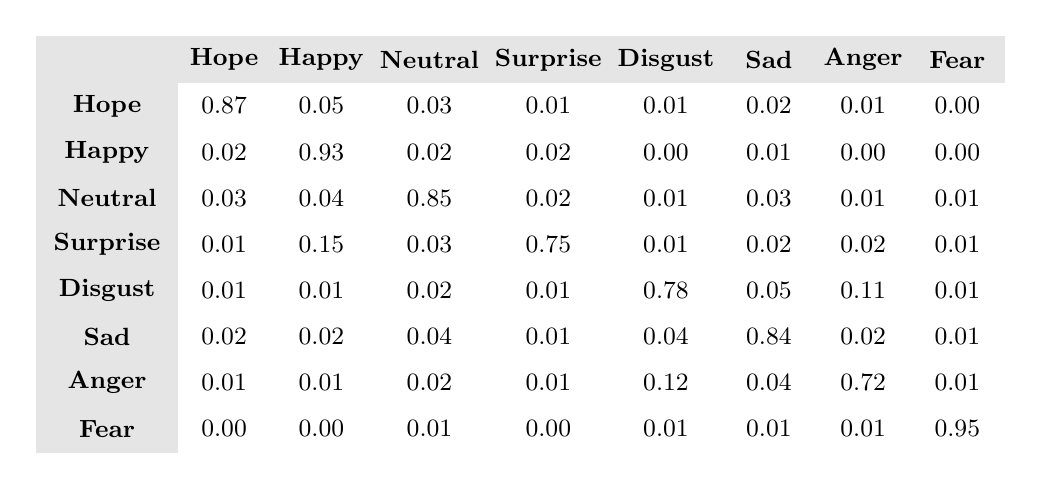
\begin{tikzpicture}
\small
% Matrix cells
\matrix (cm) [matrix of nodes, 
    nodes in empty cells,
    nodes={minimum width=1.2cm, minimum height=0.6cm, anchor=center},
    column sep=-\pgflinewidth, 
    row sep=-\pgflinewidth,
    row 1/.style={nodes={fill=gray!20, font=\bfseries\small}},
    column 1/.style={nodes={fill=gray!20, font=\bfseries\small, minimum width=1.8cm}},
]{
& \textbf{Hope} & \textbf{Happy} & \textbf{Neutral} & \textbf{Surprise} & \textbf{Disgust} & \textbf{Sad} & \textbf{Anger} & \textbf{Fear} \\
\textbf{Hope}    & 0.87 & 0.05 & 0.03 & 0.01 & 0.01 & 0.02 & 0.01 & 0.00 \\
\textbf{Happy}   & 0.02 & 0.93 & 0.02 & 0.02 & 0.00 & 0.01 & 0.00 & 0.00 \\
\textbf{Neutral} & 0.03 & 0.04 & 0.85 & 0.02 & 0.01 & 0.03 & 0.01 & 0.01 \\
\textbf{Surprise} & 0.01 & \cellcolor{orange!30}0.15 & 0.03 & 0.75 & 0.01 & 0.02 & 0.02 & 0.01 \\
\textbf{Disgust} & 0.01 & 0.01 & 0.02 & 0.01 & 0.78 & 0.05 & \cellcolor{orange!30}0.11 & 0.01 \\
\textbf{Sad}     & 0.02 & 0.02 & 0.04 & 0.01 & 0.04 & 0.84 & 0.02 & 0.01 \\
\textbf{Anger}   & 0.01 & 0.01 & 0.02 & 0.01 & \cellcolor{orange!30}0.12 & 0.04 & 0.72 & 0.01 \\
\textbf{Fear}    & 0.00 & 0.00 & 0.01 & 0.00 & 0.01 & 0.01 & 0.01 & \cellcolor{green!30}0.95 \\
};
\end{tikzpicture}
\caption{Confusion matrix: Surprise→Happy (15\%), Anger↔Disgust (11-12\%), Fear (95\%).}
\label{fig:confusion}
\end{figure}

\item \textbf{The Surprise Bottleneck:} ``Surprise" remains the most challenging 
class (0.75 F1). The confusion matrix confirms systematic confusion where 
high-valence surprise (e.g., \textfarsi{شدم زده شگفت واقعا} [I was really surprised]) is  predicted as "Happy"  with 15\% probability. This 
indicates that without specific cultural markers for shock, the model defaults 
to the underlying positive valence of the expression.
\end{itemize}

\begin{table}[htbp]
\centering
\caption{Per-class F1-score progression: Baseline vs. Augmented Proposed Method.}
\label{tab:class_f1}
\begin{tabular}{@{}lccc@{}}
\toprule
\textbf{Emotion Class} & \textbf{Baseline F1} & \textbf{Augmented F1} & \textbf{Improvement (\%)} \\ \midrule
Fear & 0.143 & 0.946 & +80.3\% \\
Happy & 0.736 & 0.928 & +19.2\% \\
Hope & 0.531 & 0.868 & +33.7\% \\
Neutral & 0.443 & 0.851 & +40.8\% \\
Sad & 0.468 & 0.840 & +37.2\% \\
Disgust & 0.217 & 0.785 & +56.8\% \\
Surprise & 0.457 & 0.754 & +29.7\% \\
Anger & 0.323 & 0.718 & +39.5\% \\ \bottomrule
\end{tabular}
\end{table}
\subsection{Training Efficiency and Dynamics}
We observed that the augmented model converged faster than the baseline. While the 3,932 seed required 4 epochs to reach peak Macro-F1, the augmented 400k model reached its best state in 3 epochs. This suggests that the synthetic samples not only balanced the distribution but also provided clearer decision boundaries for the Transformer backbone. The reduction in final loss (from 1.89 to 0.49) further underscores the stability gained through scaling and augmentation.
\subsection{Ethical Considerations}
All data was collected from publicly available Telegram channels and YouTube 
comments. No private messages or protected content was accessed. User 
identifiers were removed during preprocessing. We acknowledge that emotion 
classification in conflict zones carries risks of misinterpretation, 
particularly for high-arousal negative emotions like Fear and Anger. Our 
models are intended for aggregate social analysis, not individual-level 
prediction.

\section{Conclusion}

We demonstrated that a semi-supervised pipeline effectively bridges the resource 
gap for Dari. Scaling a 3,932 expert-labeled seed to a $\approx$ 400k corpus improved 
accuracy from 50.57\% to 85.75\%. Targeted augmentation proved critical for 
the Fear class (F1: 0.143 $\rightarrow$ 0.946). The ``Hope" category (0.868 F1) 
validates our culturally-informed approach, distinguishing aspirational 
discourse from general happiness.

Our results show that data-level augmentation complements model-level 
weighting: despite a 357x class weight, Fear F1 remained at 0.30 without 
augmentation, but reached 0.946 with 9,000 synthetic samples. This confirms 
that for extremely rare classes, augmentation provides the semantic density 
that loss weighting alone cannot.

We acknowledge: (1) single annotator without inter-annotator agreement; 
(2) systematic confusion between ``Surprise" (0.75 F1) and ``Happy" (15\% 
cross-confusion). However, multi-seed experiments (41-45) confirmed 
result stability with variance below 0.5\%. Future work includes expanding 
augmentation to Surprise and Anger classes and releasing the DEEP-Dari 
corpus as a benchmark. 
\newpage
\small
\bibliographystyle{splncs04}
\bibliography{iiWAS2026_Dari_Emotion}


%\def\refname{References}
%\bibliography{iiWAS2026_Dari_Emotion}
% \bibliography{mybibliography}
%
%\begin{thebibliography}{8}
%\end{thebibliography}
\end{document}
